\section{Method}
\subsection{Preliminary}
\label{sec:atomic}
The fundamental unit of RACES is the \textbf{verifiable environment}. Each verifiable environment $e$ is formally defined as a four-tuple:
\begin{equation}
e = \bigl(\, G_e, f_e, D_e, V_e\,\bigr),
\label{eq:atomic_env}
\end{equation}
where the components are defined as follows: 
\textbf{(1) Input sampler} $G_e$ programmatically yields valid input instances from $\mathcal{X}_e$, providing an unlimited stream of training data for each environment.
\textbf{(2) Output mapper} $f_e : \mathcal{X}_e \to \mathcal{Y}_e$ produces a unique output for any valid input. $f_e$ is implemented as code and encodes the core semantics of the verifiable environment. Its domain $\mathcal{X}_e$ and codomain $\mathcal{Y}_e$ jointly define the \textsc{domain signature} $\tau_e = (\mathcal{X}_e, \mathcal{Y}_e)$, which is the primary criterion for determining whether two environments can be composed.
\textbf{(3) Problem descriptor} $D_e : \mathcal{X}_e \to \Sigma^*$\footnote{$\Sigma^*$ denotes the natural language space.} utilizes a sampled input $x \in \mathcal{X}_e$ to render the environment to a solvable problem.
\textbf{(4) Programmatic verifier} $V_e: \mathcal{Y}_e \times \mathcal{Y}_e \to \{0, 1\}$ evaluates whether a model's output matches the reference answer $f_e(x)$.

This four-tuple characterizes a family of verifiable environments capable of generating an unlimited supply of RL training data and forms the foundation of RACES. Details regarding the construction of initial environments are provided in Appendix \ref{init_envs}.

\subsection{Compositional Closure of Verifiable Environments}
\label{sec:closure}
RACES leverages the compositional closure property of verifiable environments. Two environments $e_i$ and $e_j$ with domain signatures $\tau_{e_i}=(\mathcal{X}_{e_i}, \mathcal{Y}_{e_i})$ and $\tau_{e_j}=(\mathcal{X}_{e_j}, \mathcal{Y}_{e_j})$ are composable if the codomain of the first matches the domain of the second, that is, $\mathcal{Y}_{e_i}=\mathcal{X}_{e_j}$. Their composition is defined as:
\begin{equation}
(f_{e_j}\circ f_{e_i})(x)
=
f_{e_j}\bigl(f_{e_i}(x)\bigr),
\qquad x\in \mathcal{X}_{e_i}.
\label{eq:pairwise_composition}
\end{equation}
Because both mappers are deterministic, the composite $f_{e_j}\circ f_{e_i}$ is also deterministic, mapping $\mathcal{X}_{e_i}$ to $\mathcal{Y}_{e_j}$. Consequently, the composite maintains the same domain-codomain interface as the initial environment and can be further composed with additional environments.
More generally, a domain-compatible sequence $(e_1,\ldots,e_t)$ induces a composite mapper
\begin{equation}
F_{\pi_t}
=
f_{e_t}\circ f_{e_{t-1}}\circ \cdots \circ f_{e_1},
\label{eq:composite_mapping}
\end{equation}

with domain signature $(\mathcal{X}_{e_1},\mathcal{Y}_{e_t})$. If another environment $e'$ satisfies $\mathcal{X}_{e'}=\mathcal{Y}_{e_t}$, the composite can be recursively extended by $f_{e'}\circ F_{\pi_t}$.
This compositional closure enables RACES to expand a finite set of environments into a substantially larger space.
In practice, domain matching serves as a proposal mechanism rather than a guarantee of validity. The quality filtering process is detailed in Section \ref{sec:construction}.

\begin{figure}
    \centering
    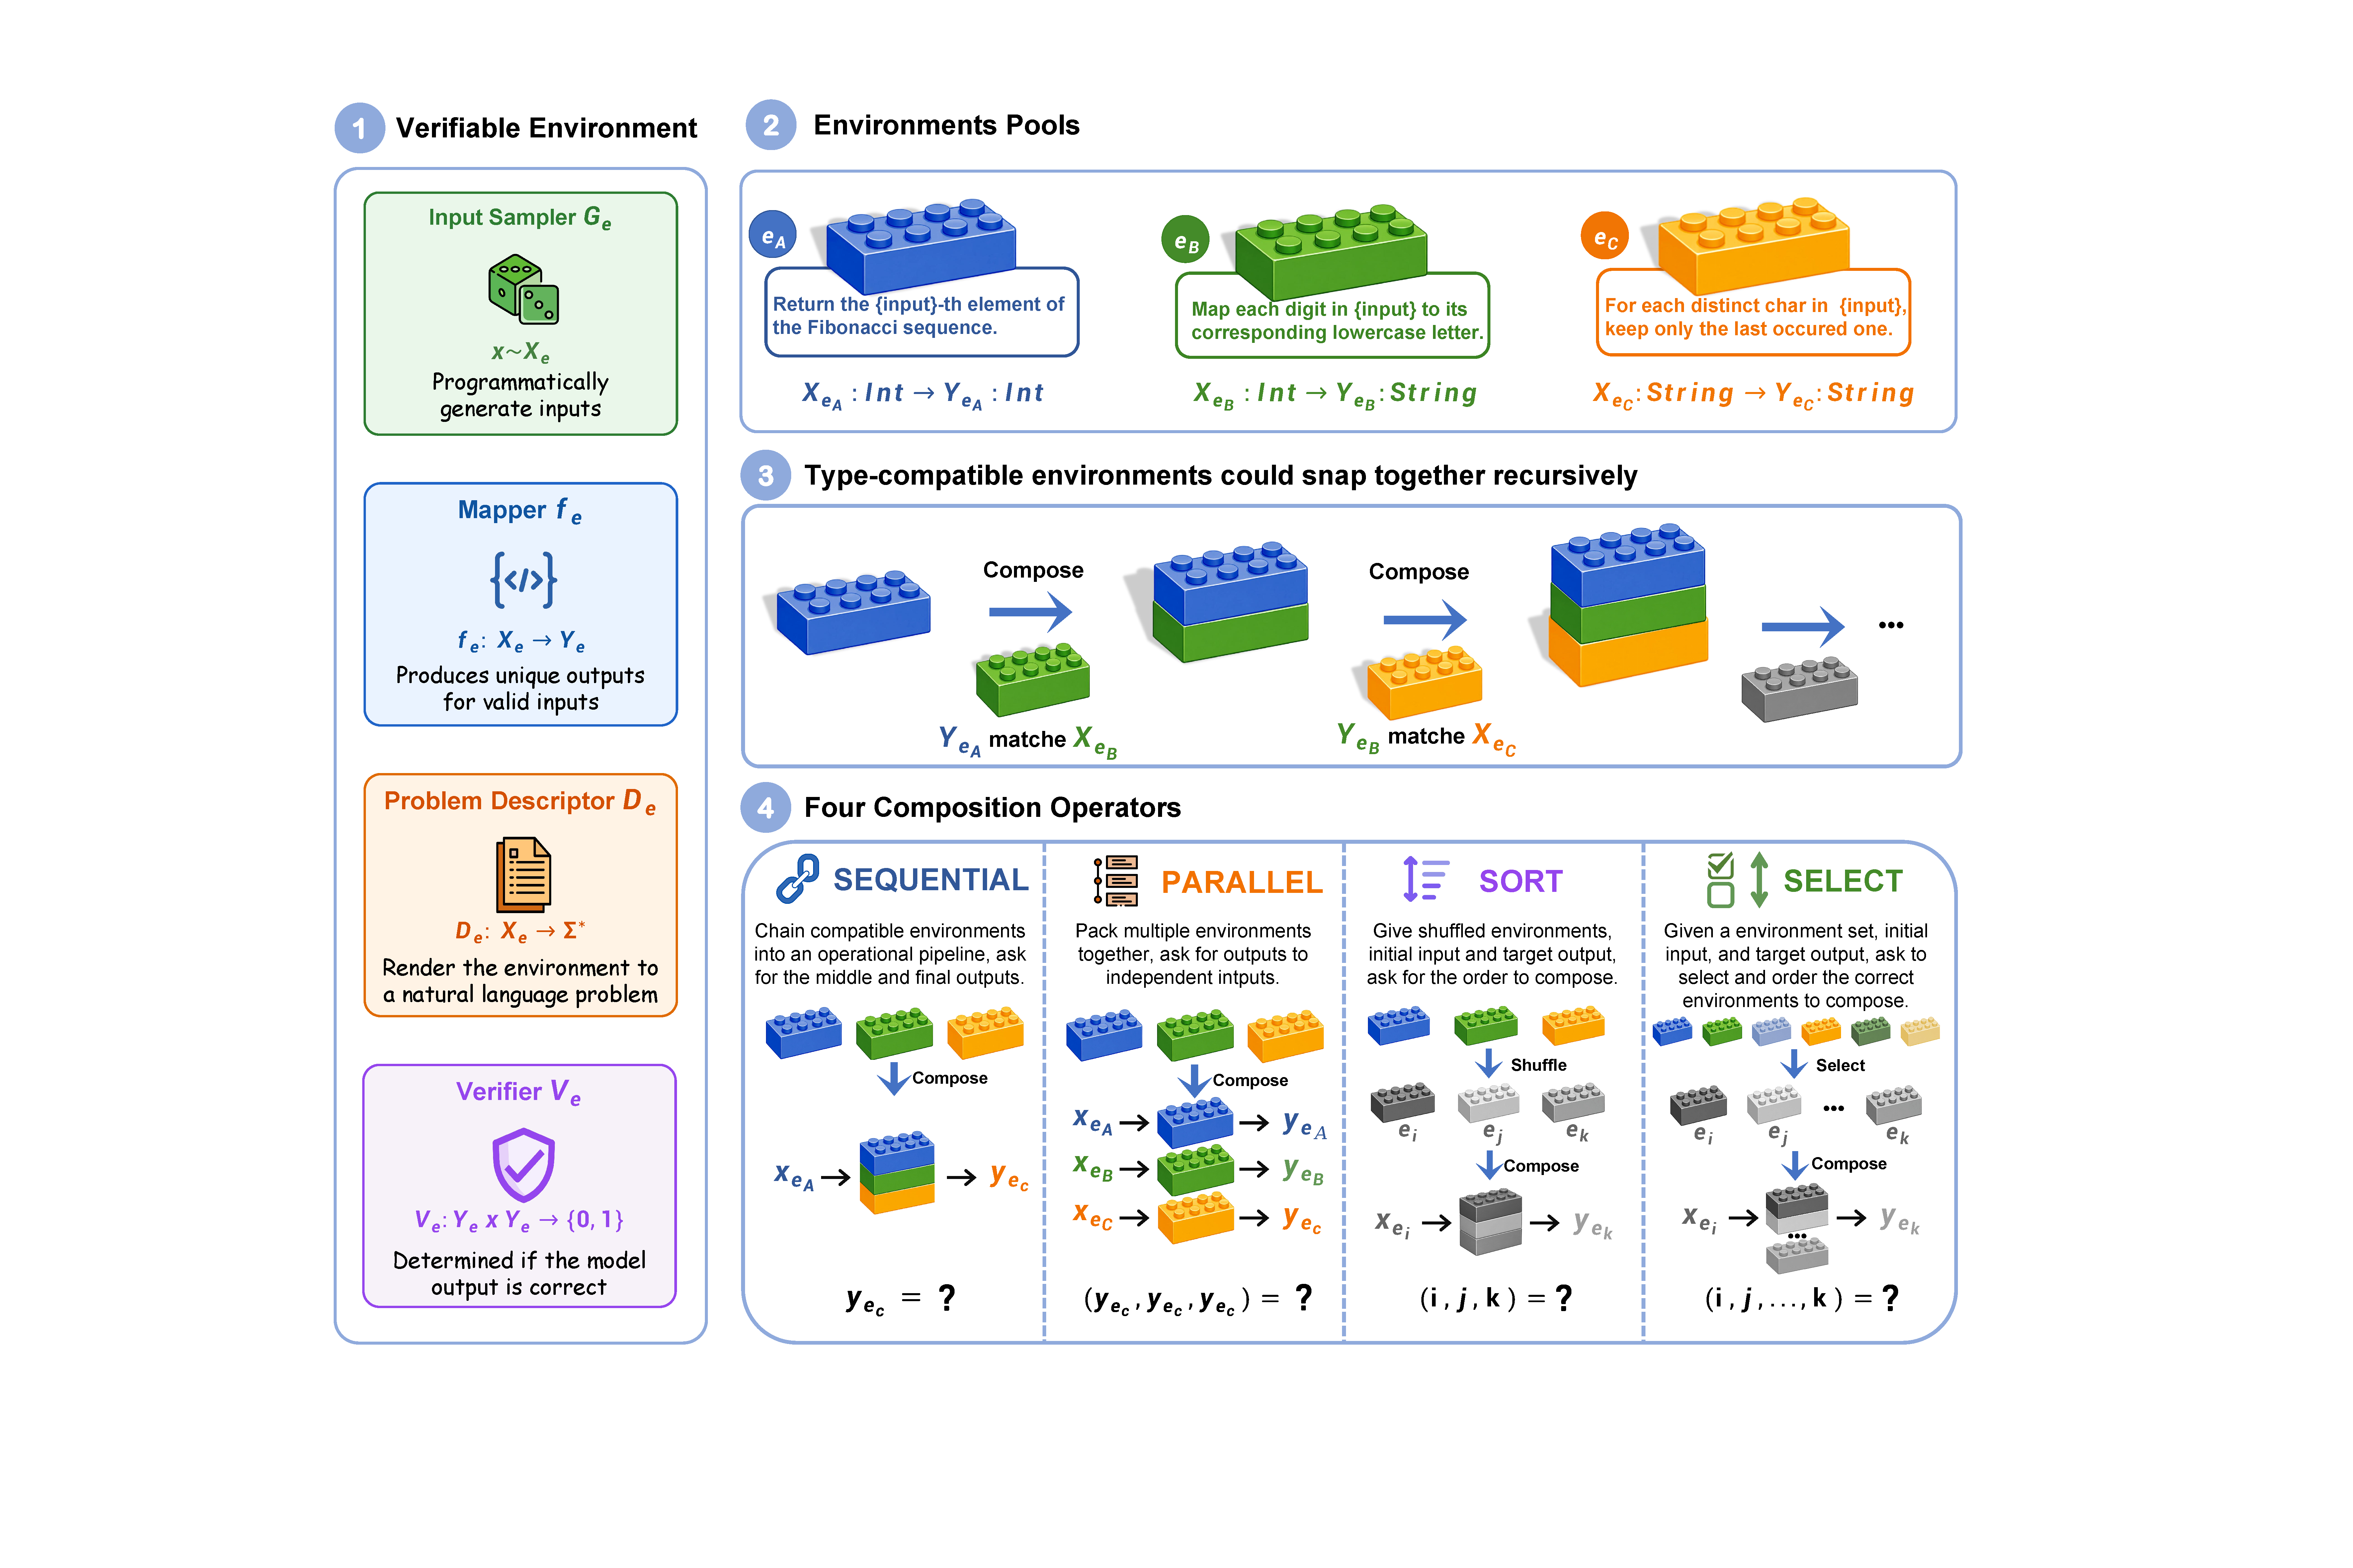
\includegraphics[width=0.9\linewidth]{Figures/method.pdf}
    \caption{Overview of the RACES framework. 1) RACES standardizes the format of a verifiable environment, which consists of four components. 2) Following the standard interface, RACES constructs a pool of verifiable environments. 3) RACES can snap environments together like Lego bricks if the codomain of one matches the domain of another. 4) RACES implements four composition operators, resulting in diverse composite patterns and reasoning requests.}
    \label{fig:lego}
\end{figure}

\subsection{Implementation of Recursive Composition}
\label{sec:construction}

To operationalize compositional closure, RACES recursively constructs composite environments through a frontier-based search strategy.
Given an environment pool, RACES automatically assembles executable composite environments at scale and renders these as model-facing RL instances.
The construction process comprises three stages: composition path discovery, quality assurance, and operator instantiation.

\paragraph{Composition path discovery.}
Given an initial input $x_0$ and an environment pool $\mathcal{E}$, RACES searches over domain-compatible composition paths. All valid continuations form a search tree rooted at $x_0$: each node is a state value and each outgoing edge an environment whose domain matches that state. A length-$t$ path is represented as
\begin{equation}
\pi_t = (x_0;\ e_1,\ldots,e_t;\ y_1,\ldots,y_t),
\qquad y_i=f_{e_i}(\mathcal{Y}_{i-1}),\quad y_0=x_0,
\label{eq:path}
\end{equation}
yielding the composite mapper $F_{\pi_t}$ defined in Eq.~\eqref{eq:composite_mapping}. At each frontier state $y_t$, RACES retrieves all domain-compatible candidates $\mathcal{C}(y_t)=\{e\in\mathcal{E}:X_e=\operatorname{type}(y_t)\}$ and executes each on $y_t$. If execution succeeds and the output passes the later quality checks, the extended path
\begin{equation}
\pi_{t+1}=\mathrm{extend}(\pi_t, e)=(x_0;\ e_1,\ldots,e_t,e;\ y_1,\ldots,y_t,f_e(y_t))
\label{eq:path_extension}
\end{equation}
is added to the frontier for further extension.
RACES implements the search as a randomized breadth-first traversal, constrained by maximum composition depth, per-execution time limits, and a cap on extensions per frontier state. Each environment is assigned a usage budget, and candidates are sampled with probabilities weighted by remaining budgets to promote balanced utilization of the pool.

\paragraph{Quality assurance.}
Domain compatibility is a necessary but insufficient condition for effective composition.
Because each $f_e$ is implemented as executable code, a domain-compatible extension may still fail on specific intermediate states due to runtime exceptions, step-limit violations, timeouts, or invalid outputs.
RACES therefore applies online executable filtering during composition path discovery, retaining only those extensions that execute successfully and yield well-formed intermediate states.
This step ensures that the constructed composites are both domain-compatible and executable, making them suitable for programmatic verification. The complete criteria are provided in Appendix~\ref{app:quality}.

\paragraph{Operator instantiation.}
After trajectory discovery and quality assurance, RACES obtains a pool of executable composite environments that are not yet formatted as model-facing training problems.
A composition operator transforms a composite environment into a model-facing problem by specifying the presented information, required model predictions, and the verification process. A single composite environment can support multiple operators, resulting in distinct reasoning patterns without redefining the composition. The composition size $t$ directly measures task difficulty, as longer paths require the model to track additional intermediate states and mitigate error accumulation. RACES samples operator-specific sizes and applies balanced sampling to prevent the training set from being dominated by a narrow range of path lengths.

\subsection{Composition Operators}
\label{sec:operators}

As shown in Figure \ref{fig:lego}, RACES implements four representative operators: SEQUENTIAL, PARALLEL, SORT, and SELECT.

\paragraph{SEQUENTIAL}
Given $x_0$ and the ordered descriptors $(D_{e_1},\ldots,D_{e_t})$, the model predicts all intermediate outputs $(\hat y_1,\ldots,\hat y_t)$. The reward rewards the longest correct prefix:
\begin{equation}
K = \min\left(\{i\in\{1,\ldots,t\}:V_{e_i}(\hat y_i,y_i)=0\}\cup\{t+1\}\right)-1, \qquad R^{\mathrm{Seq}}=\frac{K}{t},
\label{eq:seq_reward}
\end{equation}
This reward structure captures the causal dependency in chained execution, where an error at any step invalidates all subsequent outputs.

\paragraph{PARALLEL}
PARALLEL evaluates the model's ability to maintain multiple independent computational threads within a shared context.
This operator samples $n$ independent environment-input pairs $(e_i,x_i)$ and asks the model to solve them jointly within a single context. The reward is computed as the average of individual verifications:
\begin{equation}
R^{\mathrm{Par}} = \frac{1}{n}\sum_{i=1}^{n}V_{e_i}(\hat y_i,y_i).
\label{eq:parallel_reward}
\end{equation}

\paragraph{SORT}
The model receives $x_0$, the terminal output $y_t$, and a shuffled set of environment descriptors, and must output a permutation $\hat{\sigma}$ of $\{1,\ldots,t\}$. The verifier executes the predicted order from $x_0$, and the reward is
\begin{equation}
R^{\mathrm{Sort}} = 
\begin{cases}
1, & \text{if } \bigl(f_{e_{\hat{\sigma}(t)}} \circ \cdots \circ f_{e_{\hat{\sigma}(1)}}\bigr)(x_0) = y_t, \\
0, & \text{otherwise.}
\end{cases}
\label{eq:sort_reward}
\end{equation}
Non-canonical but correct orderings also receive credit under this reward scheme.

\paragraph{SELECT}
SELECT requires the model to identify both the correct subset and the appropriate ordering. The path is augmented with distractors sampled from domain-compatible alternatives encountered during the search process:
\begin{equation}
\mathcal{A}_{\pi} = \{e_1,\ldots,e_t\} \cup \mathcal{B}_{\pi},
\label{eq:select_candidates}
\end{equation}
where $\mathcal{B}_{\pi}$ denotes the distractor set. Because the distractors are themselves executable on intermediate states, they are harder than random negatives. Given $x_0$, $y_t$, and $\mathcal{A}_{\pi}$, the model outputs an ordered sequence of distinct candidates $\hat{\sigma}=(\hat{\sigma}_1,\ldots,\hat{\sigma}_k)$ with each $\hat{\sigma}_i\in\mathcal{A}_{\pi}$. The reward is
\begin{equation}
R^{\mathrm{Sel}} = 
\begin{cases}
1, & \text{if } \bigl(f_{\hat{\sigma}_k} \circ \cdots \circ f_{\hat{\sigma}_1}\bigr)(x_0) = y_t, \\
0, & \text{otherwise.}
\end{cases}
\label{eq:select_reward}
\end{equation}